\chapter{\IfLanguageName{dutch}{Stand van zaken}{State of the art}}
\label{ch:stand-van-zaken}

\paragraph{Inleiding}

Objectdetectie in domeinspecifieke contexten zoals sonarbeeldvorming wordt vaak gehinderd door een gebrek aan gelabelde data. Traditioneel vereisen gesuperviseerde modellen grote hoeveelheden handmatig gelabelde gegevens om effectieve detectie en classificatie te leren. Semi-supervised en self-supervised learning bieden echter veelbelovende alternatieven door gebruik te maken van grote hoeveelheden ongesuperviseerde data om representaties te leren. Deze literatuurstudie bespreekt de huidige technieken en hun toepassing, met een specifieke focus op de unieke uitdagingen van sonardata.

\section{Objectdetectie in sonarafbeeldingen}

Objectdetectie is een tak binnen het domein van computer vision dat gericht is op het identificeren en lokaliseren van objecten binnen beelddata (zoals foto's en video's). Dit wordt gebruikt in verschillende domeinen, zoals beveiligingssystemen (bv. om inbrekers te detecteren) of de medische wereld (bv. om tumoren op te sporen). Door de jaren heen is objectdetectie aanzienlijk geëvolueerd dankzij de vooruitgang in Deep Learning en de grote beschikbaarheid van datasets met beeldmateriaal. \autocite{He_2016} \\

Objectdetectie combineert twee belangrijke zaken in computer vision: objectlokalisatie en objectclassificatie. Objectlokalisatie bepaalt de positie van objecten, meestal in de vorm van bounding boxes \autocite{Tompson_2015}, terwijl objectclassificatie bepaalt tot welke categorie een gedetecteerd object behoort. Samen geeft dit de mogelijkheid tot het herkennen van verschillende objecten op één foto. \\

Traditioneel worden gesuperviseerde methoden -- zoals Faster \gls{rcnn}, \gls{yolo} en \gls{ssd} -- gebruikt voor objectdetectie. \autocite{Redmon_2016} Deze modellen presteren uitstekend bij voldoende gelabelde data, maar de annotatiekosten en tijdsinvestering vormen een grote belemmering, vooral bij complexe datasets zoals sonar. Sonardata vereist namelijk gespecialiseerde kennis voor het labelen, wat de annotatie nog uitdagender maakt. \autocite{Long_2015} \\

\section{Semi-supervised learning: principes en technieken}

%TODO: Schrijven 'Semi-supervised learning: principes en technieken'
\lipsum[1-3]

\section{Self-supervised learning: principes en technieken}

%TODO: Schrijven 'Self-supervised learning: principes en technieken'
\lipsum[1-3]

\section{Vergelijking van relevante methoden}

%TODO: Schrijven 'Vergelijking van relevante methoden'
\lipsum[1-3]

\section{Overzicht van bestaande datasets en annotatietechnieken}

%TODO: Schrijven 'Overzicht van bestaande datasets en annotatietechnieken'

\subsection{Beschikbaarheid van publieke datasets}

Zoals al eerder vermeld, is er voor het trainen van een objectdetectiemodel een substantiële hoeveelheid gelabelde data nodig. Tegenwoordig worden veel datasets -- zo goed als volledig geprepareerd voor het trainen van ML-modellen -- online aangeboden onder een vrije licentie. Dit zorgt ervoor dat de datasets opnieuw gepubliceerd en hergebruikt mogen worden met weinig tot geen beperkingen. Het concept van \emph{Open Data} wordt de laatste jaren steeds populairder, aangezien onderzoek zich hoe langer hoe meer ook naar het internet verplaatst. \autocite{Murray_Rust_2008} \\

Platformen zoals \href{https://www.kaggle.com/datasets}{Kaggle} of \href{https://huggingface.co/datasets}{Hugging Face} hebben zich gespecialiseerd in het verspreiden van deze open datasets en kunnen rekenen op een hele community van gebruikers om deze datasets te uploaden naar hun platformen. Ook verschillende overheidsorganisaties en onderzoeksinstellingen maken veel van hun data openbaar. Voorbeelden hiervan zijn \href{https://data.europa.eu/}{data.europa.eu} voor het dataplatform van de Europese Unie, \href{https://data.gov.be/nl}{data.gov.be} voor het Belgische Data Portaal en \href{https://data.gov/}{data.gov} voor open data van de Amerikaanse overheid. \\

Voor datasets over niche onderwerpen zijn de mogelijkheden vaak beperkter. Dit heeft verschillende redenen: eerst en vooral zijn er minder mensen met deze onderwerpen bezig, wat de kan automatisch kleiner maakt dat ze (grote) datasets gaan verzamelen en deze publiek beschikbaar maken. Ten tweede brengt een dataset samenstellen een aanzienlijke kost met zich mee, zeker wanneer deze \textit{from scratch} gemaakt moet worden en men zich bijvoorbeeld niet kan baseren op reeds bestaande datasets. Ten derde is het vaak zo dat deze zeer gespecialiseerde datasets confidentieel moeten blijven, aangezien het bijvoorbeeld gaat over gevoelige data of data over een technologie die nog volop in ontwikkeling is.

\subsection{Problemen bij sonardatasets}

Sonardata leidt aan alle drie deze problemen. Sonardata van de zeebodem moet namelijk met een gespecialiseerde \GLS{auv} verzameld worden. Weinig bedrijven hebben een nuttige reden om de kost hiervan te kunnen rechtvaardigen. Daarnaast is er namelijk nog een hele crew en een schip nodig om dergelijk onderzoek uit te voeren. Toch zijn er organisaties die deze nood hebben aan deze data. Specifiek gaat dit dan over onderzoeksinstellingen die bepaalde dingen op de zeebodem onderzoeken. Maar ook Defensie en Marine kunnen zulke data enorm goed gebruiken voor veiligheidsdoeleinden. AUV's worden in deze context gebruikt om bijvoorbeeld zeemijnen op te sporen, in kaart te brengen en onschadelijk te maken. \\

Ook worden ze gebruikt om te patrouilleren: ze kunnen hierbij kritieke infrastructuur zoals haveningangen en zeekabels bewaken en zorgen dat deze veilig en onbeschadigd blijven. Dit brengt natuurlijk onmiddellijk het derde probleem met zich mee. Alle data die door Defensie of Marine is verzameld, is automatisch confidentieel en mag onder geen enkele voorwaarde gebruikt -- laat staan gepubliceerd -- worden voor andere doeleinden. Data van de zeebodem -- en van mijnen of kritieke infrastructuur -- is namelijk van onschatbare waarde voor een potentiële vijand. \autocite{Aubard_2024_Datasets}

\subsection{Mogelijke oplossingen}

Deels omwille van de niche, deels door de hoge kosten van de apparatuur en deels door de hoge graad van gegevensbescherming is er dus nagenoeg geen -- kwalitatieve -- sonardata vrij beschikbaar. Dit is echter ook nadelig voor verdere ontwikkeling binnen het domein. Daarom zijn er -- nog maar heel recent -- enkele initiatieven opgekomen om dit alsmaar groter wordend probleem te proberen oplossen. \\

In een artikel van \textcite{Aubard_2024_Datasets} gepubliceerd in IEEE Journal of Oceaning Engineering wordt het probleem aangehaald en worden enkele oplossingen aangereikt om om te gaan met de schaarste. Daarnaast wordt een vergelijking gemaakt van (bijna) alle sonardatasets -- die overigens nog maar heel recent publiek beschikbaar zijn. Er worden in het artikel verschillende soorten datasets voor verschillende doeleinden gepresenteerd. Zo is er een aanbod van verschillende soorten sonar, verschillende formaten van data, verschillende hoeveelheden data, verschillende types objecten in de data en data voor verschillende doeleinden (zoals classificatie, objectdetectie, segmentatie, \dots). \\

In dit onderzoek wordt de focus gelegd op objectdetectie. Hierdoor vallen er al veel datasets af. Er blijven nog zo'n 5 datasets over die mogelijks gebruikt kunnen worden. \\

\begin{table}
    \centering
    \begin{tabular}{llllll}
        \toprule
        \textbf{Dataset} & \textbf{Sonar} & \textbf{Hoeveelheid} & \textbf{Object labels} & \textbf{Jaar} \\
        \midrule
        UATD                   & FLS & 9200  & Banden, Mannequins, Dozen & 2022 \\
        SSS for Mine Detection & SSS & 1170  & Mijnen                    & 2024 \\
        SWDD                   & SSS & 7904  & Muren                     & 2024 \\
        SubPipe                & SSS & 10030 & Pijpleidingen             & 2024 \\
        UXO                    & FLS & 74437 & \Glspl{blindganger}       & 2024 \\
        \bottomrule
    \end{tabular}
    \caption[Mogelijke datasets]{\label{tab:possible_datasets} Tabel van mogelijk bruikbare datasets voor dit onderzoek.}
\end{table}

Merk op dat al deze datasets nog niet lang geleden zijn gepubliceerd, wat er op wijst dat er slechts heel recent aandacht wordt besteed aan dit specifieke probleem. Op zich zijn al deze datasets van dermate kwaliteit dat ze kunnen dienen om een objectdetectiemodel te trainen. Echter vallen bepaalde datasets buiten de scope van dit onderzoek, zoals de SWDD dataset. Deze dataset is gemaakt voor de ontwikkeling van het ROSAR-framework in een paper van \textcite{Aubard_2024_ROSAR}. Ze is echter minder geschikt om te gebruiken in dit onderzoek, aangezien het namelijk sonarbeelden die gemaakt zijn door een \gls{auv} alle havenmuren van de haven van Porto de Leixões in Portugal te laten volgen en deze af te scannen bevat. \autocite{Aubard_2024_SWDD} \\

Ook de SubPipe-dataset biedt geen echte meerwaarde voor dit onderzoek. Ze bevat namelijk beelden voor de inspectie van pijpleidingen. Echter bewijst deze dataset wel dat er door de initiatieven van de afgelopen jaren datasets ter beschikking gesteld zijn met voldoende data om een robuust model mee te trainen. SubPipe bevat ongeveer 80GB aan data, verdeeld in data voor SLAM, objectdetectie en segmentatie. Ook worden er (normale) foto's in hoge resolutie (gemaakt met een GoPro Hero 10) en annotatie/metadata in verschillende formaten meegeleverd. \autocite{Alvarez_Tunon_2024} \\

Zo blijven er nog 3 datasets over die mogelijks geschikt zijn om in dit onderzoek te gebruiken. 

\newpage

\paragraph{UATD}

De Underwater Acoustic Target Detection-dataset bevat meer dan 9000 \gls{mfls}-sonarbeelden. Ze bevat de \emph{raw} sonardata met annotatie. Er komen 10 verschillende categorieën van \emph{target}-objecten in voor, waaronder kooien, banden en cilinders. De data is -- in tegenstelling tot sommige andere datasets -- verzameld door een \gls{auv} in meren en plassen. De data komt met andere woorden uit ``de echte wereld'', wat voordelig is voor de training van modellen die in \emph{real-world}-scenario's gebruikt zullen worden. \autocite{Xie_2022}

\begin{figure}[H]
    \centering
    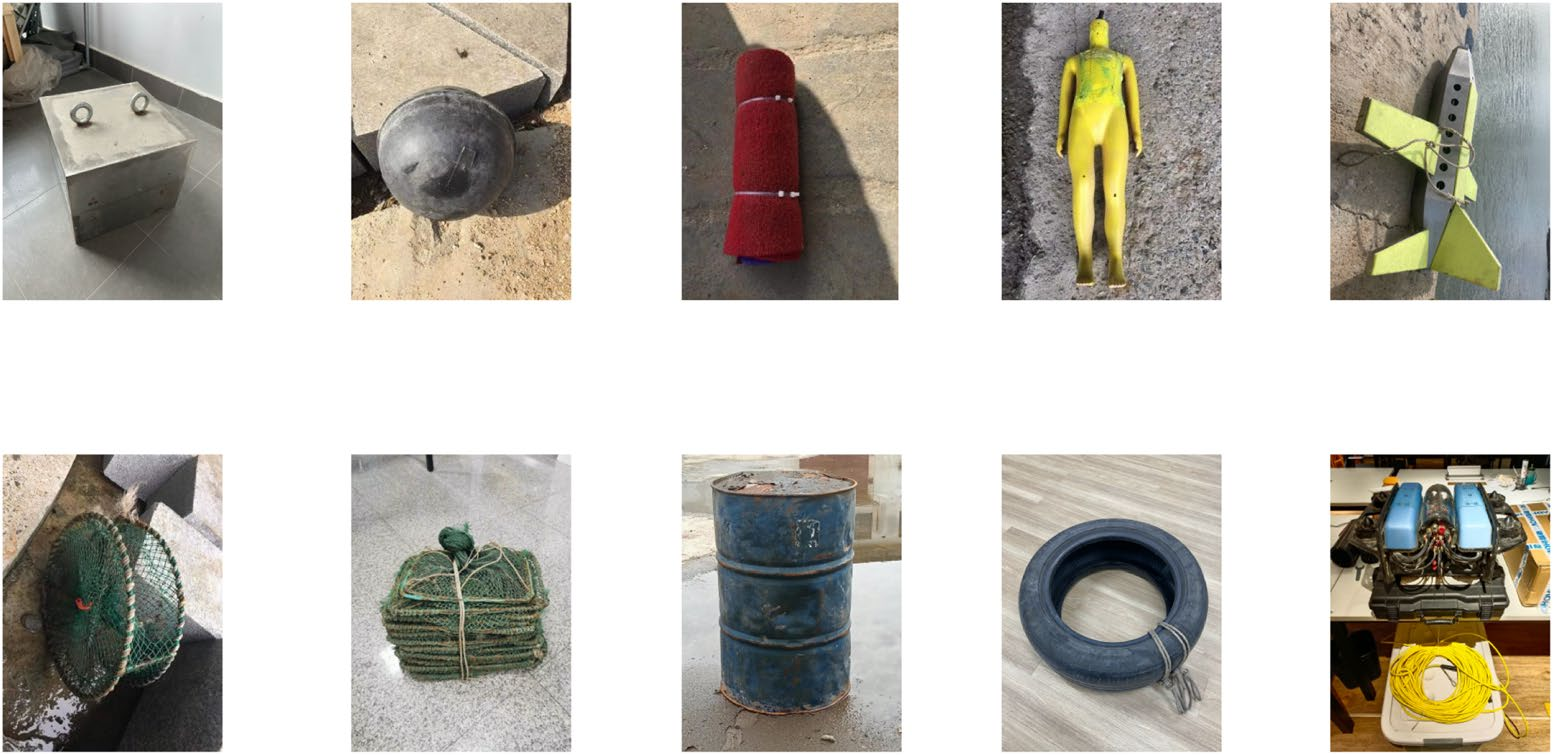
\includegraphics[width=\textwidth]{UATD_Objects.png}
    \caption[UATD Objecten.]{\label{fig:uatd_objects}Overzicht van objecten in de UATD-dataset. \autocite{Xie_2022}}
\end{figure}

De dataset wordt verspreid in een figshare-repository onder de CC BY 4.0 licentie. Deze licentie laat de gebruiker toe om het materiaal te delen en te bewerken, ook voor commerciële doeleinden. Buiten een naamsvermelding van de maker, een link naar de licentie en een vermelding of het werk al dan niet veranderd is, zijn er geen verdere restricties. De dataset wordt als ZIP-archief aangeboden. Gecomprimeerd is deze ongeveer 4,47 GB groot. Uitgepakt bevat ze drie aparte datasets en OpenSLT, de annotatietool die gebruikt werd, telkens opnieuw apart verpakt als ZIP-archief. De drie datasets zijn als volgt verdeeld: twee testsets -- \texttt{UATD\_Test\_1} en \texttt{UATD\_Test\_2} -- en één trainingsset -- \texttt{UATD\_Training}. Elk archief -- buiten die van de annotatietool natuurlijk -- bevat twee mappen: \texttt{annotations} en \texttt{images}. De map \texttt{annotations} bevat de annotaties en de map \texttt{images} bevat de sonarbeelden. \autocite{Jian_2022} \\

\begin{table}[H]
    \centering
    \begin{tabular}{llll}
        \toprule
        \textbf{Dataset} & \textbf{Aantal bestanden} & \textbf{Gecomprimeerde grootte} & \textbf{Ware grootte} \\
        \midrule
        UATD\_Test\_1  & 800  & 421.9 MB & 3.3 GB \\
        UATD\_Test\_2  & 800  & 424.6 MB & 3.3 GB \\
        UATD\_Training & 7600 & 3.9 GB   & 25.8 GB \\
        \bottomrule
    \end{tabular}
    \caption[Datasets binnen UATD]{\label{tab:uatd_datasets_overview} Tabel van eigenschappen van de datasets binnen de UATD-dataset. \autocite{Jian_2022}}
\end{table}

De bestanden volgen een vast benamingsschema zodat de beelden en de annotaties makkelijk aan elkaar gekoppeld kunnen worden. In elke dataset zijn de bestanden genummerd van \texttt{00001} tot aan het aantal bestanden in de dataset (bv. \texttt{00800} voor elke testset). Het beeld en de overeenkomstige annotatie hebben hetzelfde nummer. Zo zijn de paden voor het tweede beeld bijvoorbeeld:

\begin{itemize}
    \item \textbf{Beeld:} \texttt{UATD/UATD\_Test\_1/images/00004.bmp}
    \item \textbf{Annotatie:} \texttt{UATD/UATD\_Test\_1/annotations/00004.xml}
\end{itemize}

\begin{figure}[H]
    \centering
    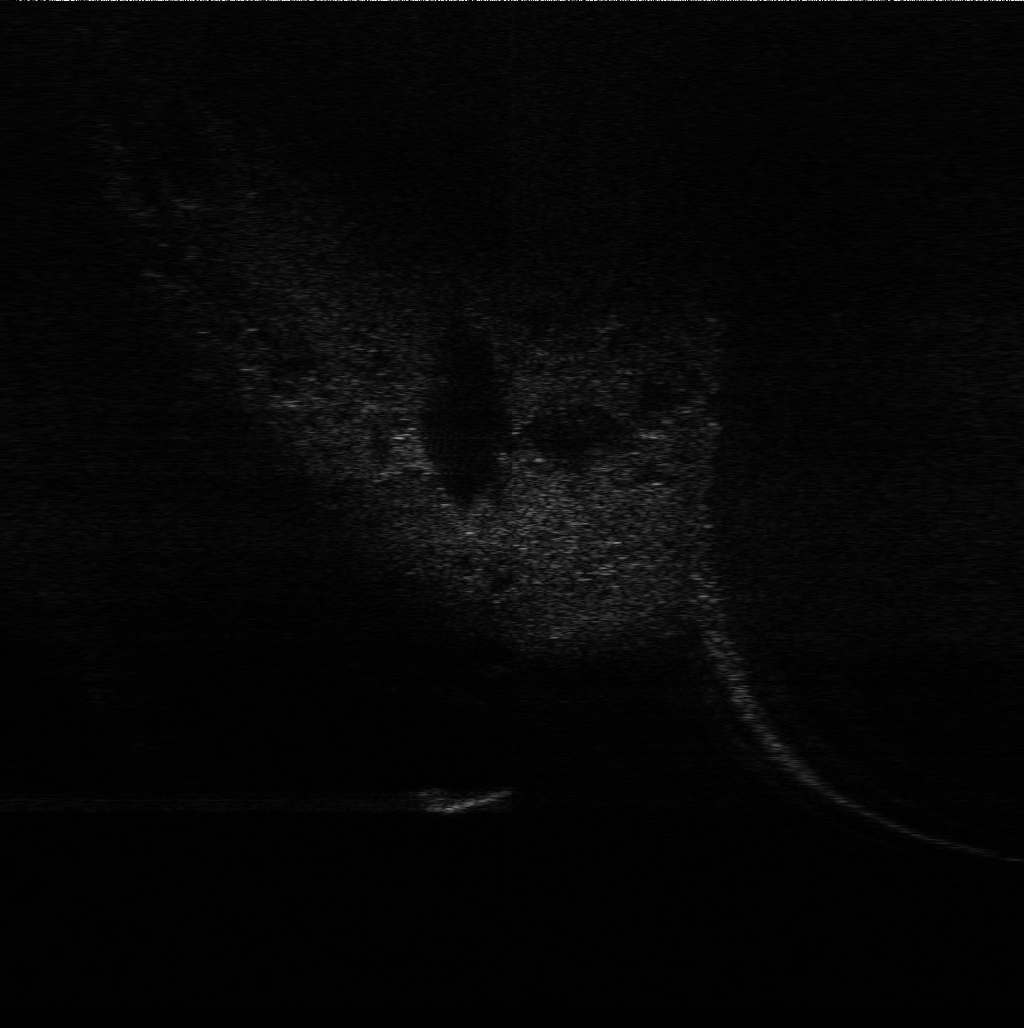
\includegraphics[width=0.5\textwidth]{UATD_example.png}
    \caption[UATD afbeelding.]{\label{fig:uatd_image}Voorbeeld van een sonarbeeld binnen de UATD-dataset (afbeelding \texttt{UATD\_Test\_1/00004}). \autocite{Xie_2022}}
\end{figure}

De beelden zijn opgeslagen als 3-kanaals ongecomprimeerde BMP-bestanden met een bitdiepte van 8 bits (één byte). Dit is één van de eenvoudigste bestandsformaten om een foto op te slaan. Het bestand bevat namelijk een lijst van alle pixels, waarbij voor elke pixel het kleur wordt bijgehouden. Het kleur wordt in dit geval dus opgeslagen in 8 bits. Dit betekent dat het kleur van elke pixel bepaald wordt door een waarde tussen 0 en 255. Aangezien er drie kanalen zijn (RGB: Rood, Groen en Blauw), wordt elke pixel dus beschreven door $8 \times 3 = 24$ bits of 3 bytes. Als de afmetingen van de afbeelding gekend zijn, is het makkelijk om de grootte van de afbeelding te berekenen met behulp van volgende formule:

$$
\text{Grootte in Bytes} = \frac{breedte \times hoogte \times \#kanalen \times bitdiepte}{8}
$$ \\

Naast enkele tientallen bytes aan header- en fotodata is dit de werkelijke grootte van een BMP-bestand. Het nadeel is echter dat zo'n bestand heel snel heel groot wordt, aangezien BMP meestal gebruikt wordt zonder compressie. Anderzijds is zo'n verzameling van BMP-bestanden dan weer heel goed te comprimeren in bijvoorbeeld een ZIP-bestand. Zo kon de UATD-dataset van ongeveer 32,8 GB naar ongeveer 4,75 GB gecomprimeerd worden \footnote{Dit gaat over de som van de drie ZIP-bestanden die nog eens gezipt in de UATD-dataset zaten. De drie bestanden zijn dus nog eens gecomprimeerd, wat de grootte van het origineel gedownloade bestand op 4,47 GB bracht.}, wat op een compressiegraad van ongeveer 6.8 neerkomt. \autocite{Bourke_1998}

\begin{figure}[H]
    \centering
    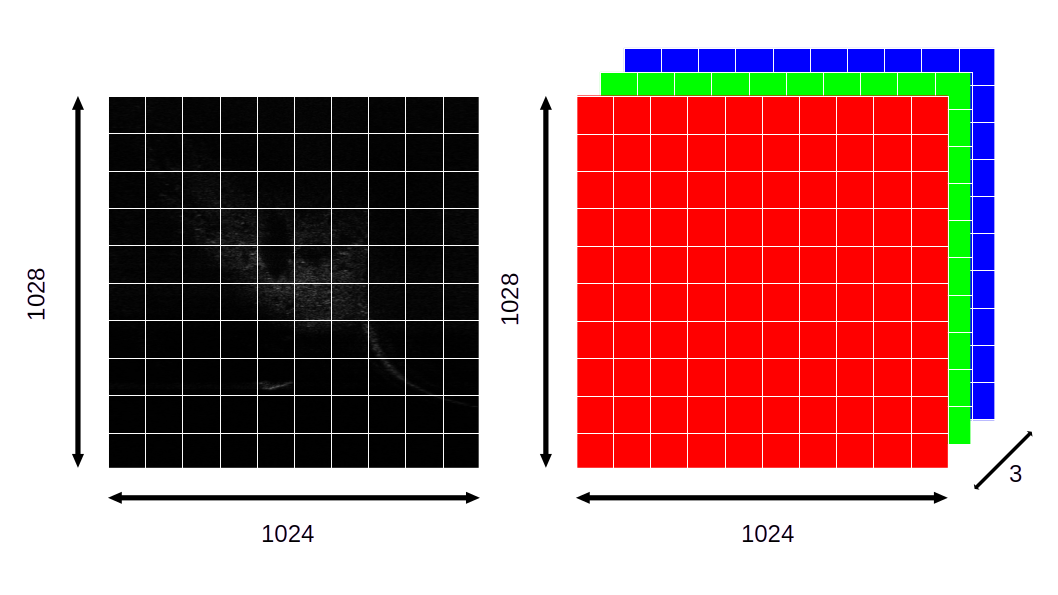
\includegraphics[width=\textwidth]{bitmap_image.png}
    \caption[Voorbeeld van een bitmap.]{\label{fig:bitmap_image}Voorbeeld van de structuur van een bitmap-afbeelding zoals BMP.}
\end{figure}

Per afbeelding is er steeds een overeenkomstig XML-bestand dat de annotatie bevat. De annotatie volgt het Pascal VOC-formaat. Dit annotatieformaat werd origineel ontwikkeld voor de Visual Object Challenge (VOC). Deze challenge is een benchmark voor classificatie en objectdetectie die sinds 2005 jaarlijks georganiseerd wordt. Ondertussen is het formaat uitgegroeid tot een veelgebruikte standaard voor de annotatie van visuele datasets voor bijvoorbeeld objectdetectie. Door het gebruik van XML is het formaat makkelijk leesbaar. Echter maken heel weinig modellen rechtstreeks gebruik van het Pascal VOC-formaat, waardoor de annotatie meestal moet omgezet worden naar een ander formaat. \autocite{Everingham_2009}

\begin{listing}[H]
    \begin{minted}{xml}
        <annotation>
            <sonar>
                <range>24.9909</range>
                <azimuth>120</azimuth>
                <elevation>12</elevation>
                <soundspeed>1498.1</soundspeed>
                <frequency>1200k</frequency>
            </sonar>
            <file>
                <folder>UATD_Test_1</folder>
                <filename>00004</filename>
            </file>
            <size>
                <width>1024</width>
                <height>1257</height>
                <channel>3</channel>
            </size>
            <object>
                <name>rov</name>
                <bndbox>
                    <xmin>574</xmin>
                    <ymin>880</ymin>
                    <xmax>618</xmax>
                    <ymax>909</ymax>
                </bndbox>
            </object>
        </annotation>
    \end{minted}
    \caption[PASCAL VOC-annotatie]{Voorbeeld van een XML-bestand met annotatie voor objectdetectie in het PASCAL VOC-formaat (annotatie van \texttt{UATD\_Test\_1/00004}). \autocite{Xie_2022}}
\end{listing}

\paragraph{SSS for Mine Detection}